\chapter{System Design: UML Diagrams}
\label{ch:uml}

This chapter presents FoodLink's design in UML~\cite{omgUml251}: the use case
diagram with scenarios, the class diagram and the activity diagram. Every
element was derived from the repository at commit \texttt{e588b35}. Actors are
the values of \code{UserRole}, use cases are implemented routes and screens,
classes are the ORM models and the matching module, and activity branches are
decisions the server takes. The earlier copies in \code{docs/uml/} predate
decisions D-50 to D-58; the diagrams here are corrected redraws, with TikZ
sources in the report's \code{diagrams/} directory.

\section{Use Case Model}
\label{sec:usecase}

\subsection{Use Case Diagram}
\label{sec:usecase-diagram}

\begin{figure}[p]
  \centering
  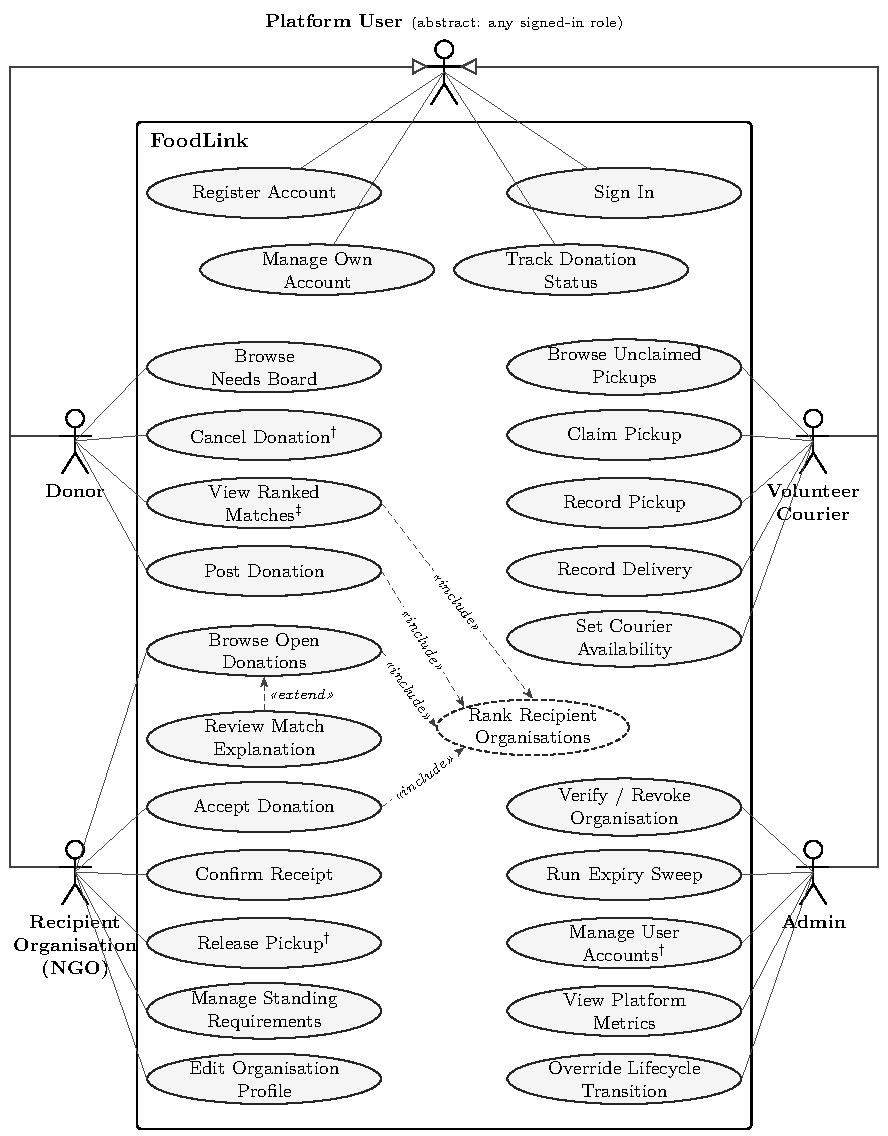
\includegraphics[width=\textwidth,height=0.9\textheight,keepaspectratio]{diagrams/use-case.pdf}
  \caption[Use case diagram of FoodLink]{Use case diagram of FoodLink.
    $\dagger$: implemented and tested in the API, not yet offered in the web
    portal. $\ddagger$: API and phone-layout camera screen only.}
  \label{fig:usecase}
\end{figure}

Figure~\ref{fig:usecase} shows four actors and 26 use cases. The actors
\emph{Donor}, \emph{Recipient Organisation (NGO)}, \emph{Volunteer Courier} and
\emph{Admin} specialise an abstract \emph{Platform User}, which carries sign-in,
account management and status tracking. \emph{Register Account} is open only to
the donor, organisation and courier roles. \emph{Post Donation}, \emph{View
Ranked Matches}, \emph{Browse Open Donations} and \emph{Accept Donation} each
$\ll$include$\gg$ the internal \emph{Rank Recipient Organisations}, and
\emph{Review Match Explanation} $\ll$extend$\gg$s \emph{Browse Open Donations}.
Some conditions are not drawn: browsing and accepting require a verified
organisation, overdue donations cannot be accepted, and donors cancel only
before pickup. \emph{Override Lifecycle Transition} represents the
administrator's place in every entry of \code{TRANSITION_ROLES} except the
courier claim.

\subsection{Use Case Scenarios}
\label{sec:scenarios}

The fifteen main use cases are specified below. Status codes are the server's
responses, and routes are relative to \code{/api}.

% ---------------------------------------------------------------------------
% A scenario is a ruled block of labelled fields; it may continue onto the
% next page. \flow numbers the main-flow steps inline.
\newcommand{\flow}[1]{\begin{enumerate*}[label=(\arabic*)]#1\end{enumerate*}}
\newenvironment{scenario}[2]{%
  \par\addvspace{8pt}\begingroup\small
  \noindent\rule{\linewidth}{0.4pt}\par\nopagebreak
  \noindent\textbf{#1 --- #2}\par\nopagebreak
}{%
  \par\endgroup
}
\newcommand{\ucfield}[2]{%
  \par\noindent\hangindent=2.5cm\hangafter=1%
  \makebox[2.5cm][l]{\textbf{#1}}#2\par}
% ---------------------------------------------------------------------------

\begin{scenario}{UC-01}{Register Account}
  \ucfield{Actor, goal}{Prospective donor, organisation or courier. \emph{Goal:} an account in a self-service role.}
  \ucfield{Pre., trigger}{Email unused; under 10 registrations per hour from the network. \emph{Trigger:} creating an account on the sign-in page.}
  \ucfield{Main flow}{\flow{\item Picks a role; enters name, email and password. \item \code{POST /auth/register} validates the email, an 8--128-character password and a self-signup role. \item The server stores a bcrypt hash and creates a courier or \emph{unverified} organisation profile. \item It returns 201 with a token.}}
  \ucfield{Alternatives}{Email exists: 409. \code{admin} role or invalid fields: 422. Over the limit: 429.}
  \ucfield{Post., rules}{Active account. An organisation is not ranked, cannot see the pool and cannot accept until verified (UC-13) and given coordinates (API only). Administrators never self-register (D-04).}
\end{scenario}

\begin{scenario}{UC-02}{Sign In}
  \ucfield{Actor, goal}{Any registered user. \emph{Goal:} an authenticated session in the right portal.}
  \ucfield{Pre., trigger}{Account exists; under 30 attempts per 5 minutes from the network. \emph{Trigger:} submitting email and password.}
  \ucfield{Main flow}{\flow{\item \code{POST /auth/login} (OAuth 2.0 password form). \item The server checks the bcrypt hash and that the account is active. \item It returns a 720-minute HS256 token, and the client opens the role's portal. \item Each later request re-reads the user.}}
  \ucfield{Alternatives}{Wrong email or password: 401 (one message). Suspended: 403. Over the limit: 429. Expired token or suspension mid-session: 401 and client sign-out.}
  \ucfield{Post., rules}{Signed in until expiry; sign-out is client-side. The token's role claim is never trusted (D-03).}
\end{scenario}

\begin{scenario}{UC-03}{Post Donation}
  \ucfield{Actor, goal}{Donor (or administrator). \emph{Goal:} offer surplus food to nearby verified organisations before it expires.}
  \ucfield{Pre., trigger}{Signed in; under 10 posts per hour for the account and 30 for the network. \emph{Trigger:} submitting \emph{Create Food Donation}.}
  \ucfield{Main flow}{\flow{\item Enters food details, address, pin, optional photo (resized in the browser) and deadline. \item \code{POST /donations} checks role, limits, field bounds and a future deadline. \item The donation is stored as \code{AVAILABLE} with an event, and organisations are ranked. \item If any is eligible, the top score is frozen and \code{MATCHED} recorded; 201 is returned.}}
  \ucfield{Alternatives}{None eligible: stays \code{AVAILABLE}. Past deadline or invalid input: 422. Over budget: 429. Organisation or courier: 403.}
  \ucfield{Post., rules}{Open to verified organisations until the deadline; nothing is assigned. Frozen score and distances are hidden from donors (D-47).}
\end{scenario}

\begin{scenario}{UC-04}{View Ranked Matches and Match Explanation}
  \ucfield{Actor, goal}{Recipient organisation; donor and administrator read the ranked list. \emph{Goal:} see how well a donation suits an organisation, and why.}
  \ucfield{Pre., trigger}{Organisation verified; donation open and not overdue. \emph{Trigger:} selecting a donation on \emph{Available Donations}, or \code{GET /donations/{id}/matches}.}
  \ucfield{Main flow}{\flow{\item \code{GET /donations} includes \code{viewerMatch}, the organisation's live \code{score_pair} result from its true position and own active needs. \item The panel shows the score, five sub-scores, distance and reasons. \item Variant: \code{/matches} lists up to 25 eligible organisations in order.}}
  \ucfield{Alternatives}{Unverified: pool not returned, with an explanation. Ineligible: no breakdown. Other readers: blurred positions, null \code{distanceKm}. Unreadable donation: 404.}
  \ucfield{Post., rules}{Read-only. Requirements affect only order and reasons (D-52); frozen and live scores differ (D-30).}
\end{scenario}

\begin{scenario}{UC-05}{Accept Donation}
  \ucfield{Actor, goal}{Recipient organisation (or an administrator for it). \emph{Goal:} take responsibility for an offered donation.}
  \ucfield{Pre., trigger}{Organisation verified; donation \code{AVAILABLE} or \code{MATCHED} and not overdue. \emph{Trigger:} \emph{Accept Donation}.}
  \ucfield{Main flow}{\flow{\item \code{POST /donations/{id}/status} with \code{ACCEPTED}. \item The server checks transition, role, deadline, own organisation and verification. \item It binds the organisation, counts one acceptance and freezes its score. \item The conditional write and event commit; the donation joins \emph{Accepted Deliveries} and the courier queue.}}
  \ucfield{Alternatives}{Overdue: 409. Unverified: 403. Another organisation accepted first: 409, changes rolled back. Another organisation's id: 403. No profile: 422.}
  \ucfield{Post., rules}{Exactly one bound organisation and one counted acceptance (D-06, D-50, D-55).}
\end{scenario}

\begin{scenario}{UC-06}{Claim Pickup}
  \ucfield{Actor, goal}{Volunteer courier. \emph{Goal:} take on collection and delivery.}
  \ucfield{Pre., trigger}{Courier profile exists; donation \code{ACCEPTED} and unclaimed. \emph{Trigger:} \emph{Accept Pickup} on \emph{Pickup Tasks}.}
  \ucfield{Main flow}{\flow{\item The queue shows food, deadline, organisation and only a coarse \code{pickupArea}. \item The courier requests \code{VOLUNTEER_ASSIGNED}. \item A conditional \code{UPDATE} binds the courier only if still \code{ACCEPTED} and unclaimed. \item The event commits; exact pin, address and donor become visible.}}
  \ucfield{Alternatives}{Another courier won: 409, ``Another courier has already claimed this pickup''. No longer \code{ACCEPTED}: 409. No courier profile: 422.}
  \ucfield{Post., rules}{Exactly one courier (D-28, D-57). Availability does not gate claiming; couriers are not verified.}
\end{scenario}

\begin{scenario}{UC-07}{Record Pickup and Delivery}
  \ucfield{Actor, goal}{The assigned courier. \emph{Goal:} record collection, then delivery.}
  \ucfield{Pre., trigger}{Donation \code{VOLUNTEER_ASSIGNED} to, or \code{PICKED_UP} by, the caller. \emph{Trigger:} \emph{Mark Picked Up}, then \emph{Mark Delivered}.}
  \ucfield{Main flow}{\flow{\item Sends \code{PICKED_UP}. \item The server checks transition and role and re-reads the donation through the courier's scope. \item The conditional write and event commit. \item \code{DELIVERED} follows the same way after handover.}}
  \ucfield{Alternatives}{Another courier's run: 404. Out of order: 409. After pickup the donor cannot cancel nor the organisation release (409).}
  \ucfield{Post., rules}{Awaits confirmation; in the courier's history from \code{DELIVERED} (D-51).}
\end{scenario}

\begin{scenario}{UC-08}{Confirm Receipt}
  \ucfield{Actor, goal}{The accepting organisation. \emph{Goal:} close the donation as received.}
  \ucfield{Pre., trigger}{Donation \code{DELIVERED} and bound to the caller. \emph{Trigger:} \emph{Confirm receipt} on \emph{Accepted Deliveries}.}
  \ucfield{Main flow}{\flow{\item Sends \code{COMPLETED}. \item The server checks transition, role and ownership. \item It increments the organisation's completions and the courier's deliveries. \item The conditional write and event commit.}}
  \ucfield{Alternatives}{Another organisation's donation: 404. Not yet delivered: 409. Donor or courier: 403.}
  \ucfield{Post., rules}{Terminal. Reliability updates for future rankings; counts towards the rescue rate if completed by the deadline.}
\end{scenario}

\begin{scenario}{UC-09}{Cancel Donation (API only)}
  \ucfield{Actor, goal}{Donor; secondary: administrator. \emph{Goal:} withdraw a donation that will not be handed over.}
  \ucfield{Pre., trigger}{Donor owns it and it is not yet \code{PICKED_UP} (an administrator may also cancel from \code{PICKED_UP}). \emph{Trigger:} status \code{CANCELLED} via the API; no portal button.}
  \ucfield{Main flow}{\flow{\item The server checks transition, role, ownership and the donor's window. \item The conditional write and \code{CANCELLED} event are applied. \item In the same transaction, a bound organisation's counted acceptance is withdrawn (never below zero).}}
  \ucfield{Alternatives}{Donor after pickup, or \code{DELIVERED}/\code{COMPLETED}: 409. Another donor: 404. A courier's pickup commits first: 409, nothing withdrawn.}
  \ucfield{Post., rules}{Terminal. Reliability is unaffected (D-58); no reason is recorded.}
\end{scenario}

\begin{scenario}{UC-10}{Release Pickup (API only)}
  \ucfield{Actor, goal}{The accepting organisation; secondary: administrator. \emph{Goal:} return a claimed pickup to the courier queue.}
  \ucfield{Pre., trigger}{Donation \code{VOLUNTEER_ASSIGNED} and bound to the caller's still-verified organisation. \emph{Trigger:} status \code{ACCEPTED} via the API; no portal button.}
  \ucfield{Main flow}{\flow{\item The server checks transition, role and ownership, treating this acceptance as a release. \item It confirms verification and the binding. \item It clears the courier without a new acceptance or re-frozen score. \item The conditional write and event commit.}}
  \ucfield{Alternatives}{Not the bound organisation: 404. Already picked up: 409. Verification revoked: 403.}
  \ucfield{Post., rules}{Unclaimed again, shown to couriers as a coarse area (D-41). Known issue: an administrator release naming another organisation counts a second acceptance.}
\end{scenario}

\begin{scenario}{UC-11}{Manage Standing Requirements and Browse Needs Board}
  \ucfield{Actor, goal}{Recipient organisation; secondary: donor. \emph{Goal:} publish needs before supply exists.}
  \ucfield{Pre., trigger}{Organisation profile exists (posting needs no verification). \emph{Trigger:} \emph{Food Requirements \& Demand Signals}; a donor opens \emph{Needs Board}.}
  \ucfield{Main flow}{\flow{\item \code{POST /requirements} with food type, quantity, unit, beneficiaries, urgency, recurrence and notes. \item \code{PATCH /requirements/{id}} edits or retires a need (\code{isActive: false}). \item Retired needs are listed with \code{includeInactive} and can be reopened. \item Donors see active needs of verified organisations.}}
  \ucfield{Alternatives}{Another organisation's id: 404. Invalid values: 422, nothing written. Explicit \code{null}: unchanged. Courier: empty list.}
  \ucfield{Post., rules}{Rows are never deleted. Active needs may break ties and add a reason, never change scores (D-29, D-44, D-52).}
\end{scenario}

\begin{scenario}{UC-12}{Edit Organisation Profile (verification-sensitive)}
  \ucfield{Actor, goal}{Recipient organisation. \emph{Goal:} keep the organisation's details correct.}
  \ucfield{Pre., trigger}{Organisation profile exists. \emph{Trigger:} saving \emph{NGO / Recipient Profile}.}
  \ucfield{Main flow}{\flow{\item \code{PATCH /recipients/me} with name, type, address, capacity, contact or phone. \item The server keeps real changes only; \code{null} clears only nullable fields. \item If a verified organisation's name, latitude or longitude changes, \code{is_verified} is cleared in the same commit. \item The page shows the result.}}
  \ucfield{Alternatives}{Non-positive capacity or out-of-range coordinates: 422. Unchanged name or other fields only: verification kept. Coordinates are API-only; clearing the pin voids verification.}
  \ucfield{Post., rules}{A voided organisation is excluded from ranking, pool and acceptance until re-verified (D-54); no self-verification (D-16).}
\end{scenario}

\begin{scenario}{UC-13}{Verify or Revoke Organisation}
  \ucfield{Actor, goal}{Administrator. \emph{Goal:} vouch for a genuine organisation, or withdraw that vouching.}
  \ucfield{Pre., trigger}{Signed in as administrator; organisation exists. \emph{Trigger:} the verify control on \emph{Partner Organizations Directory}.}
  \ucfield{Main flow}{\flow{\item The page lists organisations with verification state, reliability and the number awaiting verification. \item After checking outside the system, the administrator sends \code{POST /admin/recipients/{id}/verify}. \item The server sets \code{is_verified}; the list refreshes. \item \code{DELETE} on the same route revokes.}}
  \ucfield{Alternatives}{Non-administrator: 403. Unknown organisation: 404.}
  \ucfield{Post., rules}{Verified with coordinates: ranked, sees the pool, can accept; revoked: loses these, accepted donations unaffected. Verification is a human judgement (D-37); administrator-created organisations start verified.}
\end{scenario}

\begin{scenario}{UC-14}{Run Expiry Sweep}
  \ucfield{Actor, goal}{Administrator. \emph{Goal:} record unaccepted, overdue donations as losses.}
  \ucfield{Pre., trigger}{Signed in as administrator. \emph{Trigger:} running the sweep from \emph{Platform Donation Ledger}.}
  \ucfield{Main flow}{\flow{\item \code{POST /admin/maintenance/expire}. \item The server selects \code{AVAILABLE} and \code{MATCHED} donations past their deadline. \item It appends actor-less \code{EXPIRED} events (``Deadline passed with no recipient'') and sets the status. \item It returns the count.}}
  \ucfield{Alternatives}{Nothing overdue: count 0. Non-administrator: 403.}
  \ucfield{Post., rules}{Terminal; counted in the expiry-loss rate. Known issues: not scheduled, overdue \code{ACCEPTED} donations untouched, write not conditional.}
\end{scenario}

\begin{scenario}{UC-15}{Manage User Accounts (API only)}
  \ucfield{Actor, goal}{Administrator. \emph{Goal:} create accounts of any role; suspend, restore, rename or re-role them.}
  \ucfield{Pre., trigger}{Signed in as administrator. \emph{Trigger:} calls to \code{/admin/users}; no screen.}
  \ucfield{Main flow}{\flow{\item \code{GET} lists accounts, optionally by role. \item \code{POST} creates any role, including administrator, with its profile (organisations start verified). \item \code{PATCH /admin/users/{id}} updates \code{isActive}, \code{role}, \code{name}, \code{organization} or \code{phone}.}}
  \ucfield{Alternatives}{Duplicate email: 409. Suspending or demoting oneself or the last active administrator: 409. Unknown user: 404.}
  \ucfield{Post., rules}{Effective on the next request (a suspended user receives 401, and 403 at sign-in). The first administrator comes only from \texttt{python -m foodlink.cli create-admin} (D-04).}
\end{scenario}

\medskip
\noindent The remaining use cases in Figure~\ref{fig:usecase} are simple.
\emph{Manage Own Account} uses \code{PATCH /auth/me} and
\code{POST /auth/password}; \emph{Track Donation Status} lists donations in
one's scope with their timelines; \emph{Browse Unclaimed Pickups} is the
coarse-area queue of UC-06; \emph{Set Courier Availability} uses
\code{PATCH /volunteers/me} and is advisory; \emph{View Platform Metrics} calls
\code{GET /metrics}; and \emph{Override Lifecycle Transition} performs any
transition in Table~\ref{tab:transitions} except the claim, on a party's behalf.

\section{Class Diagram}
\label{sec:class}

\begin{figure}[p]
  \centering
  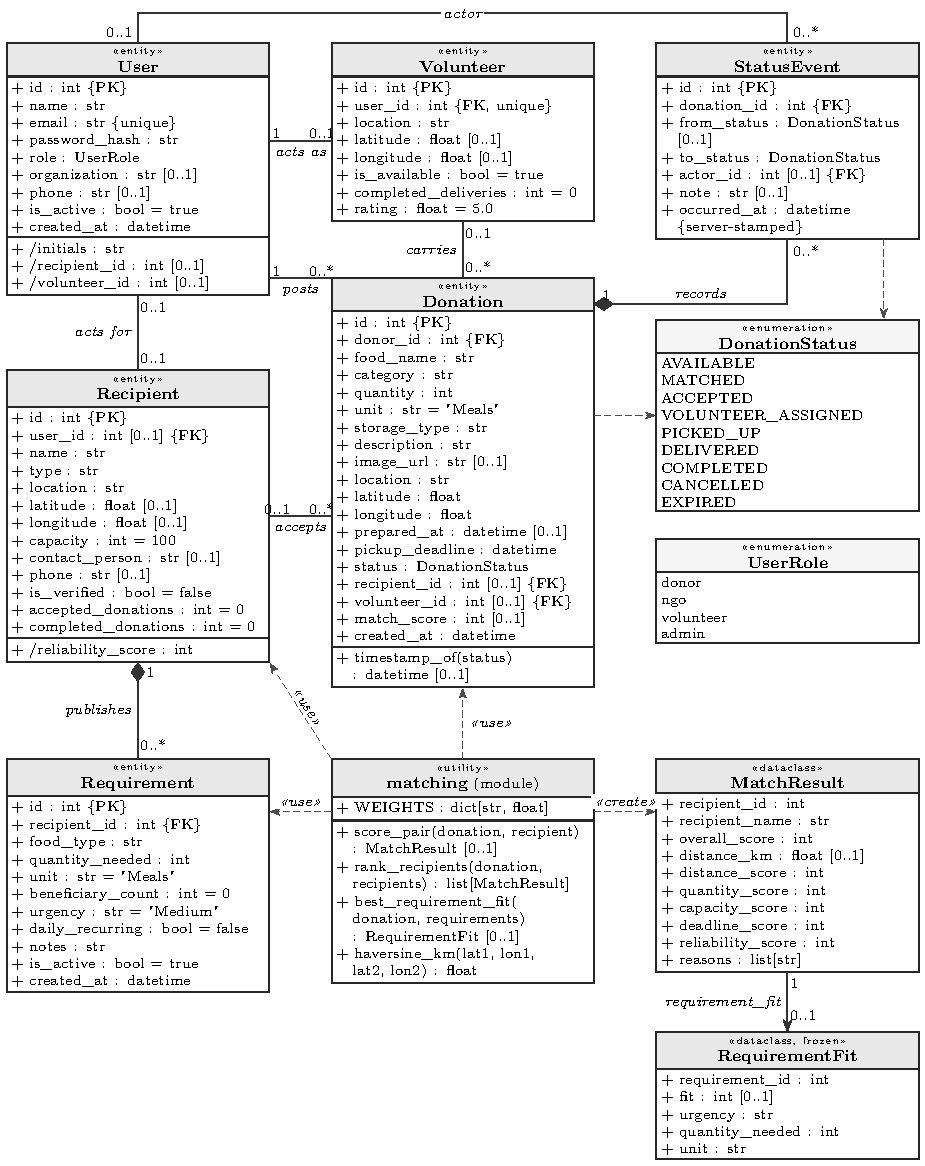
\includegraphics[width=\textwidth,height=0.9\textheight,keepaspectratio]{diagrams/class-diagram.pdf}
  \caption{Class diagram of the FoodLink domain model and matching module}
  \label{fig:class}
\end{figure}

Figure~\ref{fig:class} shows the six persistent entities and two enumerations
of \code{models.py}, and the \code{matching} module with its two data classes.
Multiplicities follow the foreign keys: a user acts for at most one
\code{Recipient} (seeded recipients have none) and at most one \code{Volunteer},
whose user key is unique and mandatory; a \code{Donation} has zero or one
recipient and courier until acceptance and claim; and a \code{StatusEvent}
optionally names its actor. \code{Donation}--\code{StatusEvent} and
\code{Recipient}--\code{Requirement} are compositions with cascading deletes,
and derived properties carry a slash (for example
\code{Recipient.reliability_score}). The matching module is a
$\ll$utility$\gg$ whose \code{MatchResult} objects are transient; only
\code{overall_score} is copied into \code{Donation.match_score}. Roles are an
enumerated attribute and profiles are associations, so there is no inheritance.

\section{Activity Diagram}
\label{sec:activity}

\begin{figure}[p]
  \centering
  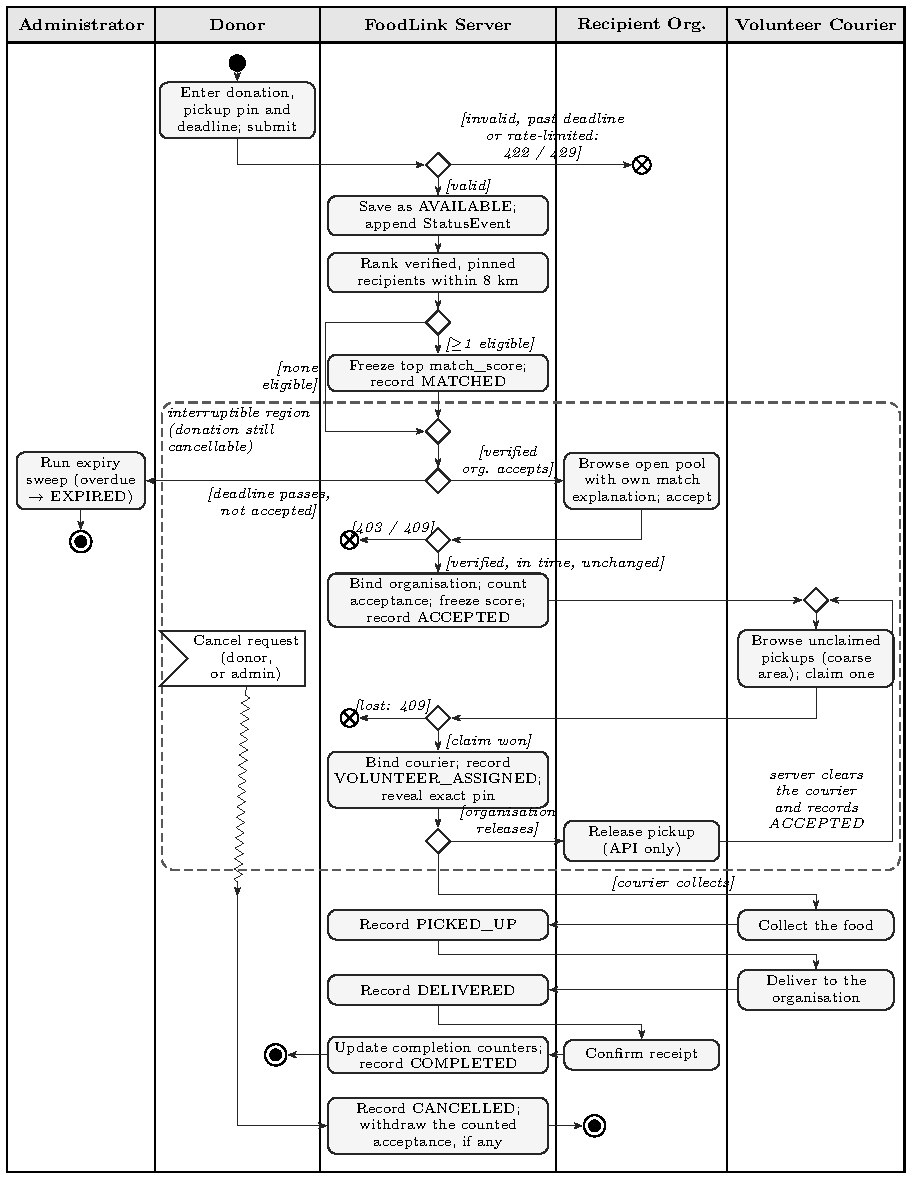
\includegraphics[width=\textwidth,height=0.9\textheight,keepaspectratio]{diagrams/activity-diagram.pdf}
  \caption[Activity diagram of the donation lifecycle]{Activity diagram of the
    donation lifecycle, from posting to completion, expiry or cancellation.
    Codes on refusal edges: 422 invalid input or past deadline; 429 rate
    limit; 403 unverified organisation; 409 overdue, already taken or claim
    lost.}
  \label{fig:activity}
\end{figure}

Figure~\ref{fig:activity} models the workflow across five swimlanes: the four
roles and the server, the only lane that records state. The main path runs
through validation, storage and ranking (\code{MATCHED} only when an
organisation is eligible), acceptance gated by verification, the deadline and a
conditional write, then a conditional courier claim, pickup, delivery and
confirmation. Refused requests end at flow-final nodes and leave the donation
unchanged. Donations nobody accepts in time end in \code{EXPIRED} through the
sweep, and an API-only release loop returns a claimed pickup to the queue. The
dashed interruptible region spans the states in which a donor may still cancel;
its interrupting edge ends in \code{CANCELLED} and withdraws any counted
acceptance. Administrator cancellation after pickup, administrator
\code{ACCEPTED}\,$\to$\,\code{EXPIRED}, and administrators acting for other
parties are omitted for readability.
